\documentclass[11pt]{article}
\usepackage{hyperref}
\usepackage{amsthm}
\usepackage{amsmath}
\usepackage{amsfonts}
\usepackage{tikz}
\usepackage{ wasysym }
\usepackage{fancyvrb}
\usetikzlibrary{arrows.meta,positioning}


\newtheorem{example}{Example}


\author{Group 16: Nicholas Jacob, Deborah Alagwu, Joyce Aladenika}
\title{Homework 5 Advanced Analytics and Metaheuristics}

\begin{document}
\maketitle

\begin{enumerate}
\item Flying
\begin{enumerate}
\item To attack this problem, you will want to minimize the cost.  This is the objective.  There are two tricky items in the formulation, the ramp fee will only turn on if no or a limited amount of fuel is taken and extra fuel must be carried as a matter of precaution.  We deal with the first as a indicator of whether we are paying the fee or not at each airport, $\delta_i$.  We identify the other variable of importance as the amount of fuel taken on at each of the airport, $x_i$.  We also add a variable for the total fuel in the jet for ease of computation, $f_i$.
\begin{eqnarray}
\min \sum_{i}\frac{x_i}{6.7}\cdot price_i + \delta_i\cdot rampfee_i\\
minfuel_i\cdot\delta_i\leq x_i\quad \forall i\in {1,\dots ,5}\\
f_0 = 7000\\
f_1 = x_1 + f_0\\
f_2 = x_2 + f_1 - fuelburn_1\\
\vdots\\
2500 + fuelburn_i \leq f_i \leq 14000\quad \forall i \in {1,\dots ,5}
\end{eqnarray}

We also account for the max takeoff weight and landing weight by including passengers and tankered fuel.  We see there are 2 passengers on the first leg, 4 on the second and 8 on all the rest.  We also consider the refilling of the plane into final ready state (7000lbs of fuel) after the final leg.

Lastly, we must turn on or off the fee for landing if we don't take the minimum fuel.  We do this with the condition,
\[
6.7minGalsToWaiveFee_i - x_i\leq M\delta_i
\]
Here we set $M = 140000$, the max amount of fuel we can take.

Here is the code and data file:


{\tiny \VerbatimInput{group_HW5_p1.mod}}


{\tiny \VerbatimInput{group_HW5_p1.dat}}

Lastly the output is below.  We pay the fee several times even when we do take on some fuel at stops.  Total cost of \$17 ,500 or so.

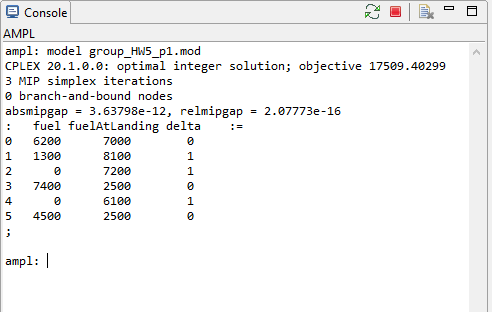
\includegraphics[width = .9\textwidth]{outputp1.png}

To make the model not allow tankering, we will change the model to require that fuel at landing be exactly the minimum 2500 (except on the 0th leg where I have already assumed it has been filled up)


{\tiny \VerbatimInput{group_HW5_p1a.mod}}

With output and new price of just above 22k.  We do pay one less landing fee in this model.

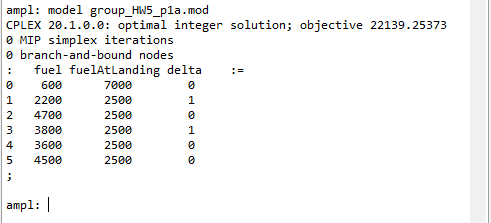
\includegraphics[width = .9\textwidth]{output1a.png}

\item  To add the condition that if we buy we must buy at least 200 gallons, we simply require that each $x_i$ is a minimum of 200 * 6.7 = 1340 lbs of fuel if it is activated.  We will use another binary for this purpose.  We need the constraint
\[
1340*\Delta_i\leq x_i\leq M\Delta_i
\]
Again we used 14000 for the $M$ value.  We show code next.  It is very similar with the few new constraints and variables.

{\tiny \VerbatimInput{group_HW5_p1b.mod}}

We see in the output below that the plan only changes slightly with this requirement and is very near our original optimal cost, about \$11 more than the original.

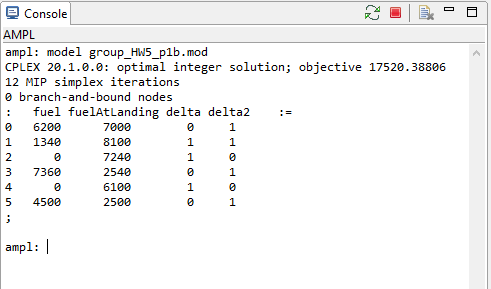
\includegraphics[width = .9\textwidth]{outputp1b.png}
\end{enumerate}

\item Following the outline \href{https://math.stackexchange.com/questions/4594715/vertex-coloring-approximation-algorithm-using-linear-programming}{here}, 
we let $H$ be the total number of exhibits possibly available.  Here we set $H = 10$ with the assumption that we will need much less. Define $w_i$ means we used that particular exhibit to house animals.  $x_{v,i}$ means we used $i$ exhibit to house $v$ animal.  Then our goal is to:
\begin{equation}
\begin{array}{cl}
minimize\ & \sum_{i=1}^H w_i\\
s.t.& \sum_{i=1}^Hx_{i,v} = 1\quad \forall v\\
& x_{i,v} + x_{i,u} \leq w_i\quad \forall (v,u)\in Table, \ i\leq H\\
&x_{i,v},w_i\in \{0,1\}
\end{array}
\end{equation}

Let's take a moment to explain the constraints.  The first constraint requires that each animal is only in one pen.  The second constraint requires that two animals that do not get along cannot be in the same pen and forces the $w$ binary to turn on.  We code this into AMPL as follows:

{\tiny \VerbatimInput{group_HW5_p2.mod}}

With use of a data file:

{\tiny \VerbatimInput{group_HW5_p2.dat}}

We see the output here: 


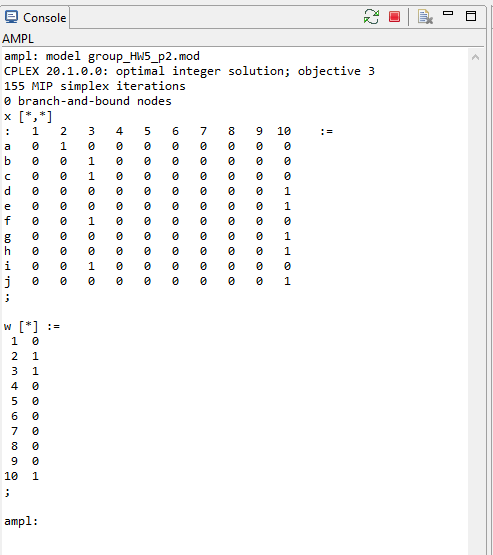
\includegraphics[width = .9\textwidth]{outputp2.png}

Interpreting the output, we see that we will require 3 pens.  Animal $a$ will live alone.  Animals $b$, $c$, $f$, and $i$ will live in the next pen.  Animals $d$, $e$, $g$, $h$ and $j$ will live together in the last pen.  We have no idea why AMPL selected the second third and tenth pen but that should not matter to our minimization of the total number of pens required.

\item For our approach to this problem, we create two variables, $\delta_{a,i}$ and $x_{a,i}$.  $a$ is the type of fuel and $i$ is the tank number.  Our binary $\delta$ describes which type of fuel our tank will use and the real positive$x$ describes how many 1000L will be moved of each type of fuel into that tank.    Our objective is to minimize the cost of pumping the fuel into tanks without mixing the fuel types.  
\[
minimize\ \sum_{a \in types, i \in tanks} cost(a,i)\cdot x_{a,i}
\]
The conditions follow
\begin{equation}
\begin{array}{cl}
s.t. & \sum_{a \in types} \delta_{a,i} \leq 1\\
&\sum_{i \in tanks} capacity(i)\cdot \delta_{a,i}\geq totalAvailable(a)\\
&\sum_{a \in types} 1000\cdot x_{a,i} \leq capacity(i)\\
&\sum_{i \in tanks} 1000\cdot x_{a,i} = totalAvailable(a)\\
& \delta_{a,i} \leq x_{a,i} \leq M\delta_{a,i}
\end{array}
\end{equation}
The first constraint requires only one type of oil be used in any tank.  The second requires that enough capacity is reserved for each type of oil.  The next requires that you don't put more oil than capacity into any one tank.  The next requires that all oil find a home in one of the tanks.  The last requirement activates $\delta$.  If you move any oil into the tank, the binary is turned on.

We code this into AMPL below:

{\tiny \VerbatimInput{group_HW5_p3.mod}}

We see the output here:


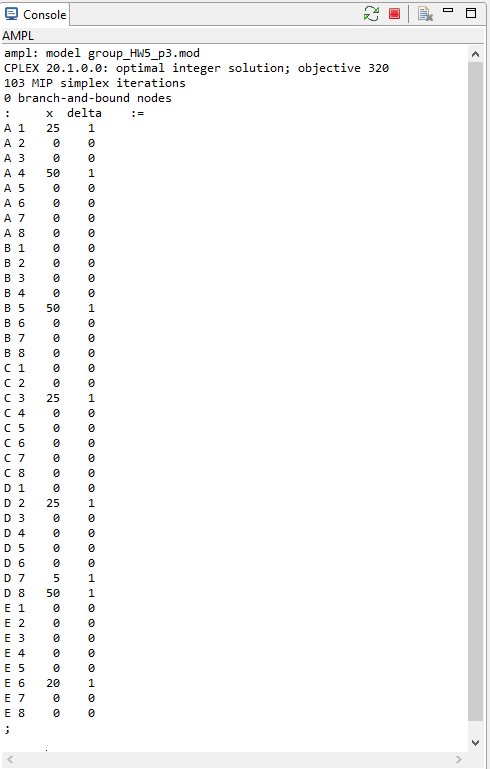
\includegraphics[width = .9\textwidth]{outputp3.png}

We see the total cost of \$320.  We use tank 1 and 4 for type A fuel, tank 5 for type B, tank 3 for type C, tanks 2, 7, and 8 for type D and tank 6 for type E.  This is quite the haphazard plan.  I could only imagine the field agents complaining about how the engineers have no idea what they are doing.  We see an important assumption here that labour was not considered here in this plan.    Someone will have to run this storage plan and then later undo it.  This could cost the company more than if we had implemented a simpler plan.
\item We code the piecewise linear cost function in the method described in the modules and text.  Each piece of the cost function gets a variable representing it and the total is forced by the some of each.  We force them to turn on in order by careful use of binary variables associated with when each of the levels has been filled.  For spacerays we do this with 4 levels ($sr$) and three binaries ($srb$).  They are related as
\begin{equation}
\begin{array}{cl}
s.t. & 125srb1\leq sr1\leq 125\\
& 100 srb2\leq sr2\leq 100\cdot srb1\\
&150 srb2\leq sr3 \leq 150\cdot srb2\\
& sr4\leq 700\cdot srb3
\end{array}
\end{equation}
Each of the binaries will allow the next to turn on only after the level variable has completely filled.
We also ask that $SR = sr1+ sr2 +sr3 +sr4$ be integer.  We do the same thing for zappers.  Details are in the AMPL model file.  We also consider a plastic, labour, and total production restriction.  Lastly we demand that the number of zappers plus 350 is greater that the number of space rays.

Here is the model file:

{\tiny \VerbatimInput{group_HW5_p4.mod}}

Here is the data file:

{\tiny \VerbatimInput{group_HW5_p4.dat}}

Here is the output:


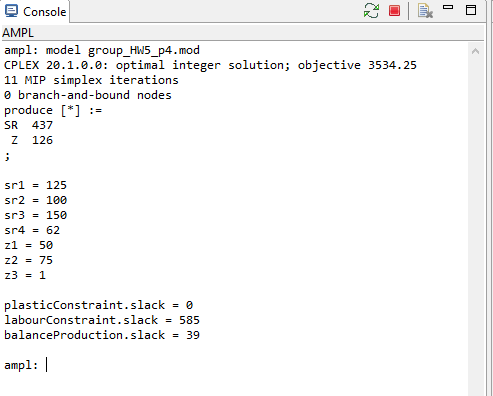
\includegraphics[width = .9\textwidth]{outputp4.png}

We create 437 space rays, 126 zappers, making \$3534.25  There is no remaining plastic but there are some more labour hours available.
   
\item To approach this problem, we first coded into AMPL the LP problem without the binary restrictions on $x_i$.  We instead insisted that $0\leq x_i\leq 1$.  We then solved the full LP problem and observed the output.  In the first bubble, we see the general solution.  Next we pick $x_1$ and force it to be binary.  We do this by adding the condition that $x_1 = 0$ and then also $x_1 = 1$.  We solve both of those with the full LP method.  We arrive at a binary solution for $x_1 = 0$ and a non-binary solution for $x_1 = 1$.  We repeat this process for $x_4$, picking $x_4$ since it was not binary in the current solution.  We find a non-binary solution and an infeasible solution.  We do not continue on the infeasible tree but do continue down the branch that gave an LP solution.  This time we examine $x_3$.  Again an infeasible solution and a solution that beats our original other binary solution.  Having no more branches to continue on, we terminate the algorithm.  We also run the algorithm in AMPL and see we did indeed find the maximum under the binary assumption.

 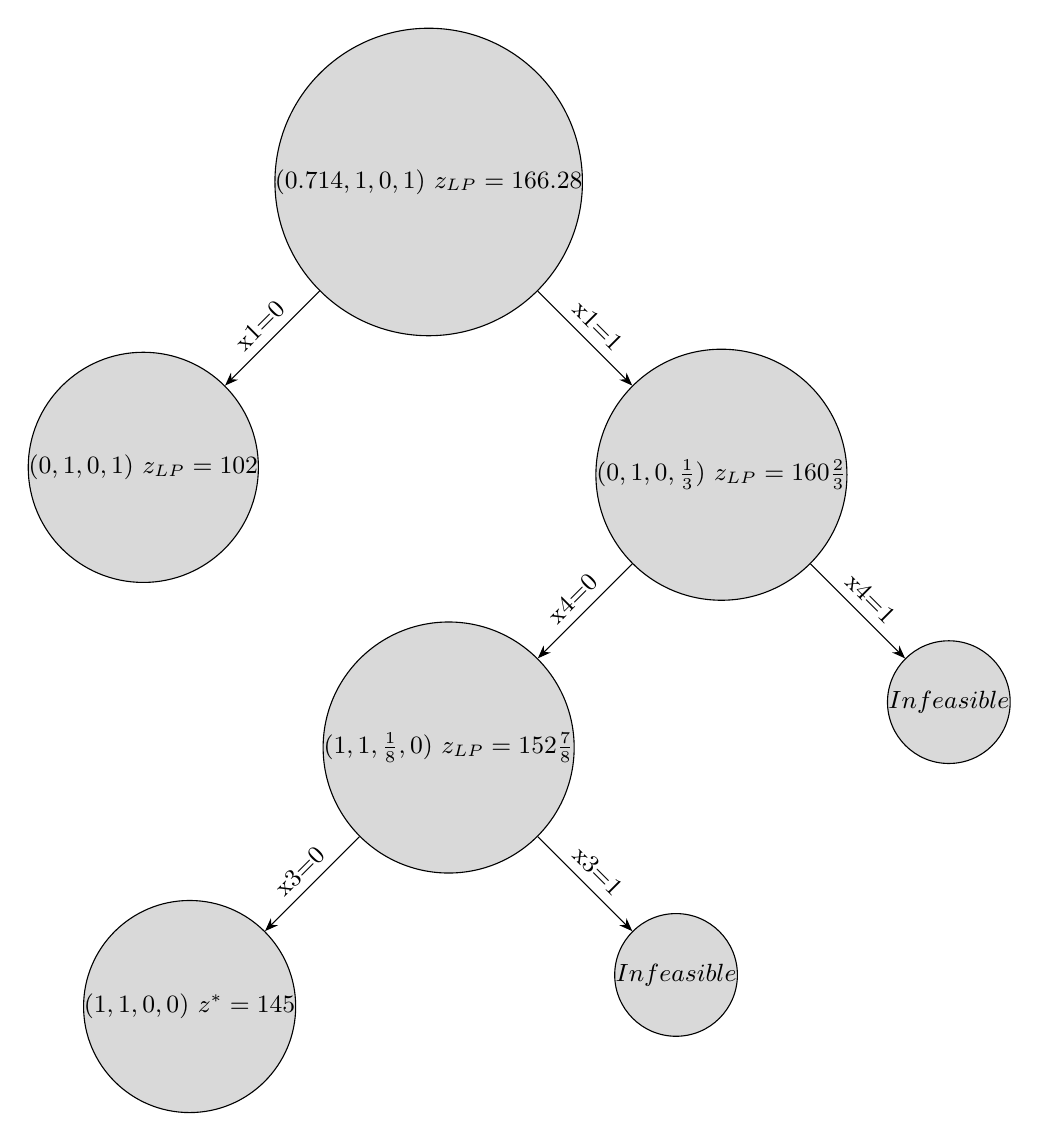
\begin{tikzpicture}[
      mycircle/.style={
         circle,
         draw=black,
         fill=gray,
         fill opacity = 0.3,
         text opacity=1,
         inner sep=0pt,
         minimum size=30pt,
         font=\small},
      myarrow/.style={-Stealth},
      node distance=1
.2cm and 1.2cm
      ]
      \node[mycircle] (0) {$(0.714,1,0,1)\ z_{LP} = 166.28$};
      \node[mycircle,below left=of 0] (1) {$(0,1,0,1)\ z_{LP} = 102$};
      \node[mycircle,below right=of 0] (2) {$(0,1,0,\frac13)\ z_{LP} = 160\frac23$};
      \node[mycircle,below left=of 2] (3) {$(1,1,\frac18,0)\ z_{LP} = 152\frac78$};
      \node[mycircle,below right=of 2] (4) {$Infeasible$};
      \node[mycircle,below left=of 3] (5) {$(1,1,0,0)\ z^* = 145$};
      \node[mycircle,below right=of 3] (6) {$Infeasible$};
      

    \foreach \i/\j/\txt/\p in {% start node/end node/text/position
      0/1/x1=0/above,
	0/2/x1=1/above,
	2/3/x4=0/above,
	2/4/x4=1/above,
	3/5/x3=0/above,
	3/6/x3=1/above}
	 %s5/buynew/7600/above}
       \draw [myarrow] (\i) -- node[sloped,font=\small,\p] {\txt} (\j);


    \end{tikzpicture}


{\tiny \VerbatimInput{group_HW5_p5.mod}}
The output is included here but is rather lengthy.

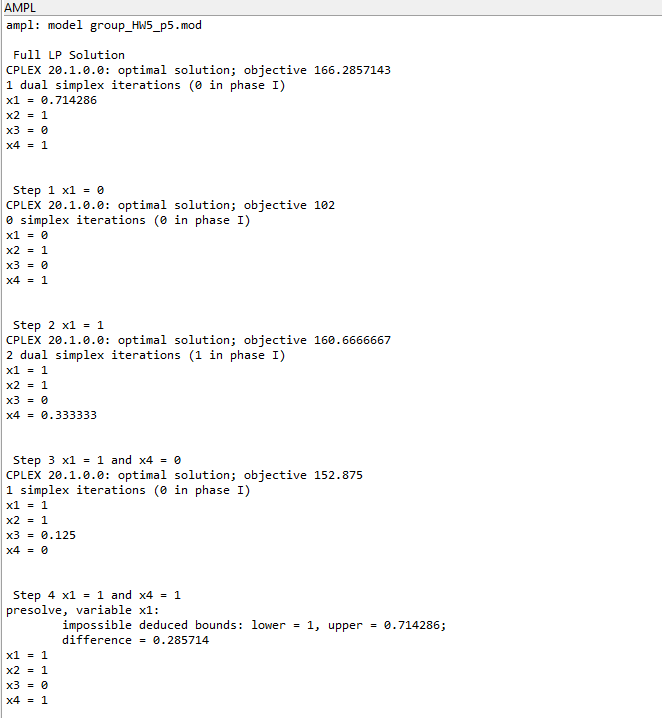
\includegraphics[width = .9\textwidth]{outputp5.png}

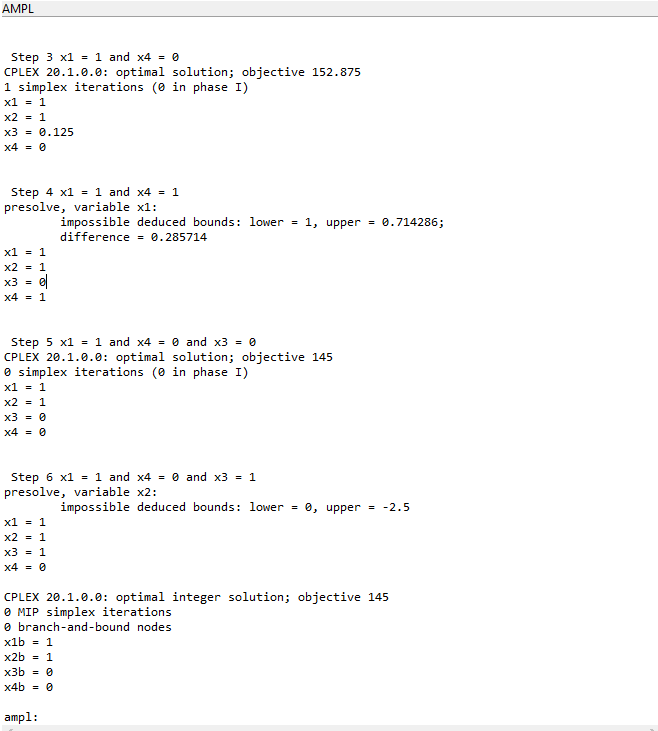
\includegraphics[width = .9\textwidth]{outputp5a.png}
\end{enumerate}



\end{document}
